\documentclass[12pt, twoside]{article}
\usepackage[letterpaper, margin=1in, headsep=0.5in]{geometry}
\usepackage[english]{babel}
\usepackage[utf8]{inputenc}
\usepackage{amsmath}
\usepackage{amsfonts}
\usepackage{amssymb}
\usepackage{tikz}
\usepackage{yhmath}
\usetikzlibrary{quotes, angles}
\usepackage{graphicx}
\usepackage{enumitem}
\usepackage{multicol}

\usepackage{venndiagram}

\title{Regents Geometry}
\author{Chris Huson}
\date{June 2022}

\usepackage{fancyhdr}
\pagestyle{fancy}
\fancyhf{}
\renewcommand{\headrulewidth}{0pt} % disable the underline of the header

\fancyhead[LE]{\thepage}
\fancyhead[RO]{\thepage \\ Name: \hspace{4cm} \,\\}
\fancyhead[LO]{BECA / Dr. Huson, Mr. Segal / Geometry\\* Unit 13: Data Analysis\\* 8 June 2022}

\begin{document}
\begin{enumerate}

\item For each Venn diagram, write an expression representing the shaded area.
\begin{enumerate}
    \item For example, for this diagram \\*
    %\\*
    \begin{venndiagram2sets}
        \fillA
        \fillB
    \end{venndiagram2sets}
    Expression:  %\\*
    \item %\\*[15pt]
    \begin{venndiagram2sets}
        \fillACapB
    \end{venndiagram2sets}
    Expression: %\\*
    \item %\\*[15pt]
    \begin{venndiagram2sets}
    \fillBNotA
    \end{venndiagram2sets}
    Expression: %\\*
    \item %\*[15pt]
    \begin{venndiagram3sets}
    \fillA
    \fillCCapB
    \end{venndiagram3sets}
    Expression: %\\*
\end{enumerate}

\item Shade the area representing $A' \cap B'$ \hspace{1cm}
    \begin{venndiagram2sets}
    \end{venndiagram2sets}


\newpage
\item Given: \\*
\qquad $A = \{a, b, c, d, e\}$
\qquad $B = \{a, e, i, o, u\}$
\begin{enumerate}
    \item What is $A \cup B$?\\*[20pt]
    \item What is $A \cap B$?\\*[20pt]
\end{enumerate}

\item Suppose there are 19 species of fruit-eating monkeys in the western hemisphere. Their diets are as follows:
\begin{itemize}
  \item 16 species of monkeys eat bananas
  \item 12 species eat apples
  \item 11 eat both apples and bananas
\end{itemize}
Complete the Venn diagram below, writing the number of species of fruit-eating monkeys in each region to represent the situation. (Use ``A" for apple, ``B" for banana)
  \begin{center}
    \begin{venndiagram2sets}[tikzoptions={scale=1.5}]
    \end{venndiagram2sets}U
  \end{center}
How many species have a diet that does not include apples nor bananas?


\item A survey question has three possible responses, $A$, $B$, and $C$. Among 100 surveys, the frequencies of the answers collected were $n(A)=40, n(B)=35, \text{ and } n(C)=25$.
\begin{enumerate}
    \item If a survey is selected at random, what this the probability the response was $B$?\\*[20pt]
    \item What is the probability a survey selected at random was an answer other than $C$?\\*[20pt]
\end{enumerate}

\newpage
\item The universal set $U$ is defined as the set of positive integers less than 13. The subsets $A$ and $B$ are defined as follows: \\*
\qquad $A =$ \{integers that are multiples of 3\}\\*
\qquad $B =$ \{prime numbers\} \\* [5pt]
(note: Prime numbers have only themselves and one as factors. One is not considered a prime.)
\begin{enumerate}
    \item List the members of $A$\\*[20pt]
    \item List the members of $B$\\*[20pt]
    \item Place the elements of $A$ and $B$ in the appropriate regions in the Venn diagram below.\\*[5pt]
        \begin{venndiagram2sets}[tikzoptions={scale=2.5}]
        \end{venndiagram2sets}U\\*
    \item List the items in the set $(A \cup B)^\prime $\\*[20pt]
    \item If an element is selected at random, what is the probability that it is a member of the set $A \cap B$?
\end{enumerate}

\newpage
\item Let $f(x) = x^2+x-2$ and $g(x)=x+2$
\begin{enumerate}
    \item Rewrite $f$ in vertex form and state the vertex as an ordered pair.\\*[35pt]
    \item Factor the function $f$ and write down its roots.\\*[35pt]
    \item Graph the function $f$, labeling it. Mark the intercepts and graph the axis of symmetry as a dotted line, labeling it with its equation.
    \item Graph $g$ and label it with its name or equation.
    \item Mark the intersections of $f$ and $g$ as ordered pairs.

\end{enumerate}


\begin{figure}[!htbp]
\begin{center}
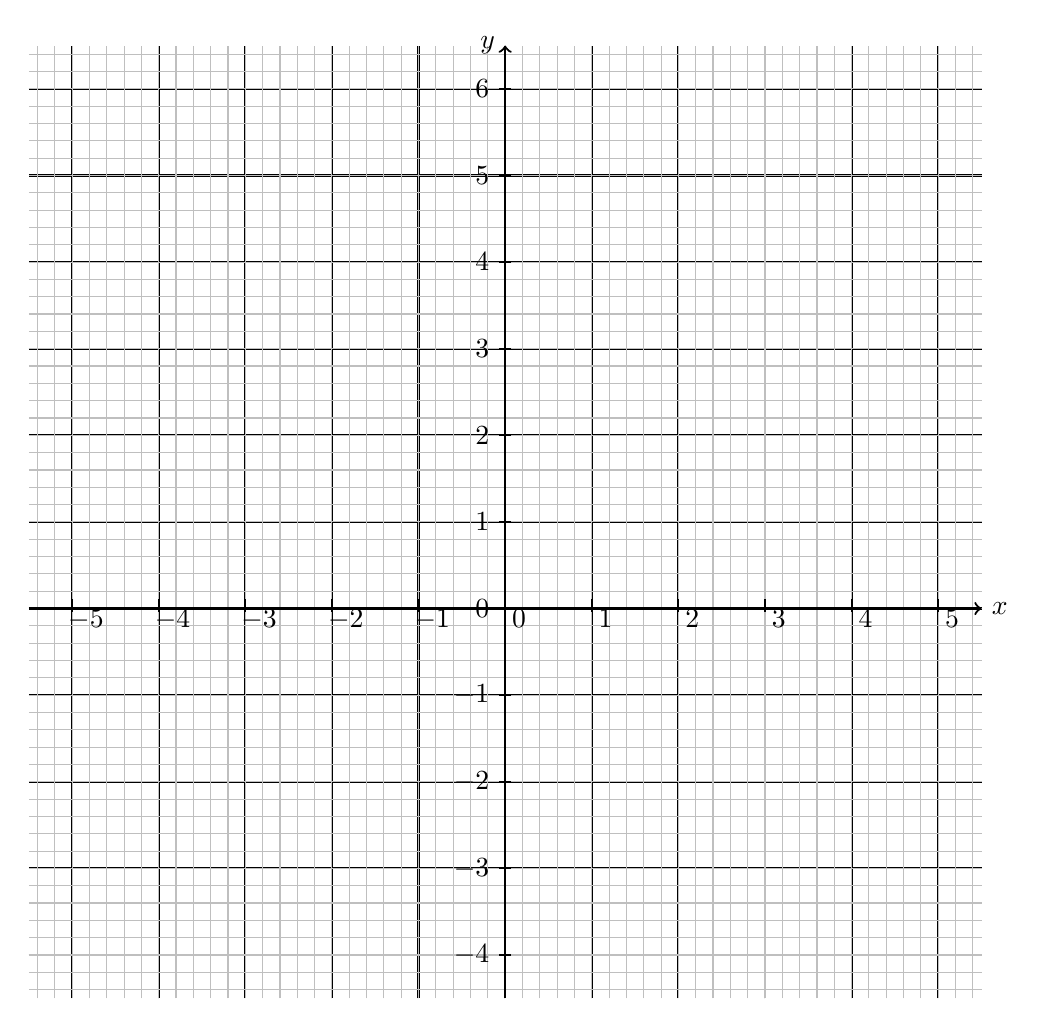
\begin{tikzpicture}[scale=1.1]

%grid
\draw [thick, color=black,, xstep=1.0cm,ystep=1.0cm] (-5.5,-4.5) grid (5.5,6.5);
\draw [thin, color=lightgray,, xstep=0.2cm,ystep=0.2cm] (-5.5,-4.5) grid (5.5,6.5);

\foreach \x in {-5, -4, -3, -2, -1, 0,1,2,3,4,5}
\draw[shift={(\x,0)},color=black] (0pt,-1pt) -- (0pt,3pt) node[below]  {$\quad \x$};

\foreach \y in {-4, -3, -2,-1,0,1,2,3,4, 5, 6}
\draw[shift={(0,\y)},color=black] (2pt,0pt) -- (-2pt,0pt) node[left]  {$\y$};

\draw [thick, ->] (-5.5,0) -- (+5.5,0) node [right] {$x$};
\draw [thick, ->] (0,-4.5) -- (0,6.5) node [left] {$y$};

%\draw [<-, ->] plot[domain= -3.5:2.5] (\x, \x*\x +\x -2);
%\draw [<-, ->] plot[domain= -5.5:3] (\x, \x+2);

\end{tikzpicture}
\end{center}
\end{figure}

\newpage
Simplify, leaving no negative or fractional exponents.

\item $2x^{-3}y \times \frac{1}{4}x^2 y^{-1}$\\*[45pt]
\item $\displaystyle a^{\frac{3}{4}} \times (\frac{\sqrt{a}}{b^4})^{\frac{1}{2}}$\\*[55pt]
\item $\ln{e^4}$\\*[35pt]
\item $\log 5^2 + \log 4$\\*[55pt]
\item $(2x^2-x-5)(x-3)-(x^2+3x-5)(2x-3)$\\*[85pt]
\item Factor the expression and then solve for $x$: $2x^3-2x^2-24x=0$

\newpage
\item Let $f(x) = 2x -5$ and $g(x)=(x-1)^2$
\begin{enumerate}
    \item Find $(f \circ g)(x)$\\*[65pt]
    \item Find $f^{-1}(x)$\\*[65pt]
\end{enumerate}

\item The function $f(x)=e^x$ is shown on the graph. Sketch $g(x)=f(x-2)+3$. Plot and label the asymptote(s).

\begin{figure}[!htbp]
\begin{center}
\begin{tikzpicture}

%grid
%\draw [thick, color=black,, xstep=1.0cm,ystep=1.0cm] (-5.5,-1.5) grid (5.5,16.5);
%\draw [thin, color=lightgray,, xstep=0.2cm,ystep=0.2cm] (-5.5,-1.5) grid (5.5,16.5);

\foreach \x in {-5, -4, -3, -2, -1, 0,1,2,3,4,5}
\draw[shift={(\x,0)},color=black] (0pt,-3pt) -- (0pt,3pt) node[below]  {$\x$};

\foreach \y in {-1,0,1,2,3,4,5, 6, 7}
\draw[shift={(0,\y)},color=black] (2pt,0pt) -- (-2pt,0pt) node[left]  {$\y$};

\draw [thick, ->] (-5.5,0) -- (+5.5,0) node [right] {$x$};
\draw [thick, ->] (0,-1.0) -- (0,7.5) node [left] {$y$};

\draw [<->] plot[domain= -3.5:2] (\x, e^\x);

\end{tikzpicture}
\end{center}
\end{figure}

\end{enumerate}

\end{document}


\item The events $A$ and $B$ are independent with $\mathrm P(A)=0.4$ and $\mathrm P(B)=0.3$.
\begin{enumerate}
    \item What is $\mathrm P(A \cap B)$?\\*[20pt]
    \item What is $\mathrm P(A \cup B)$?\\*[20pt]
\end{enumerate}

\item The events $A$ and $B$ are mutually exclusive with $\mathrm P(A)=0.5$ and $\mathrm P(B)=0.2$.
\begin{enumerate}
    \item What is $\mathrm P(A \cap B)$?\\*[20pt]
    \item What is $\mathrm P(A^\prime \cup B)$?
\end{enumerate}


\item Using a calculator, find how many sets of three elements can be selected from a set of 10, when order does not matter, i.e. $_{10}\mathrm C_3$. \\*[20pt]

\item On May 5th, 20 horses will compete in the Kentucky Derby, ``the most exciting two minutes in sports."  Among the twenty horses, how many possible finishes of first, second, and third place are possible?
